\documentclass[11pt, a4paper, oneside]{memoir}                                                      %%

\usepackage[utf8]{inputenc}
\usepackage[ngerman]{babel}     % new german spelling, umlauts and other regional settings like date format
\usepackage[shortlabels]{enumitem}
\usepackage{nameref,zref-xr}
\zxrsetup{toltxlabel}
\usepackage{graphicx}           % allow for inclusion of images
\usepackage[table,svgnames]{xcolor} % define colors
\usepackage{url}                % weblinks, etc.
\usepackage{colortbl}           % colored table cells
\usepackage{longtable}          % tables, which are longer than one page
\usepackage{hyperref}
\usepackage[intlimits]{mathtools}
\hypersetup{
	bookmarksopen=true,                       % expand bookmark tree in acrobat by default
	pdftitle={SEPMP},                         % set title in meta pdf information
	pdfauthor={Teilnehmer 1, Teilnehmer 2, Teilnehmer 3},                             % set author in meta pdf information
	pdfsubject={},                            % set subject in meta pdf information
	pdfkeywords={},                           % set keyword list in meta pdf information
	colorlinks=true,                          % use colored links instead of black ones
	linkcolor=blue,                           % color for internal links
	anchorcolor=black,                        % color for anchor links
	citecolor=black,                          % color for bibliography links
	filecolor=magenta,                        % color for system local links
	urlcolor=blue,                            % color for url links
	plainpages=false,                         % must be false, so that PDF bookmarks work properly
	hypertexnames=false,                      % use guessable names for links; used for correct bookmarks
	linktocpage                               % link page numbers in toc instead of section names
}

% Keine Numerierung
\setsecnumformat{}
\def\sectionmark#1{\markboth{#1}{#1}}

\begin{document}

    \makeatletter
    \newcommand{\mysubject}{Plannungsbericht}
    \newcommand{\mygroup}{Gruppe 9}
    \newcommand{\myauthor}{
        Ivana Drazovic \\
        Merveille Kana Tsopze Mafo \\
        Aurelle Daine Pellahe Wafo \\
        Emilia Schreiner \\
        Justus Will
    }
    \makeatother

    \thispagestyle{empty}
	\newcommand{\Rule}{\rule{\textwidth}{0.5mm}}
	\begin{center}
        % upper part
        \vspace{0.5em}
        {\Large AG Computergrafik \& HCI \\ apl. Prof. Dr. Achim Ebert \par}
        \vspace{0.5em}
        {\Large SEP/MP \the\year \par}
        \vspace{5cm}

        % middle part
        \Rule
        \vspace{1cm}
        {\Huge Exploding Kittens \par}
        \vspace{0.5em}
        {\Large \mysubject \par}
        \vspace{0.5em}
        {\small \today \par}
        \vspace{0.7cm}
        \Rule

        \vfill %%%%%%%%%%%%%%%%%%%%%%%%%%%%%%%%%%%%%%%%%%%%%%%%%%%%%%%%%%%%%%%%

        % lower part
        \emph{\textbf{\mygroup}} \\[1em]
        \myauthor
	\end{center}

    \newpage
    \tableofcontents
    \newpage

    \section{Analysemodel}
        Zuerst wurde mittels eines Analysemodels die benötigten Klassen und deren Verbindung ermittelt.

        \begin{figure}[h]
			\centering
			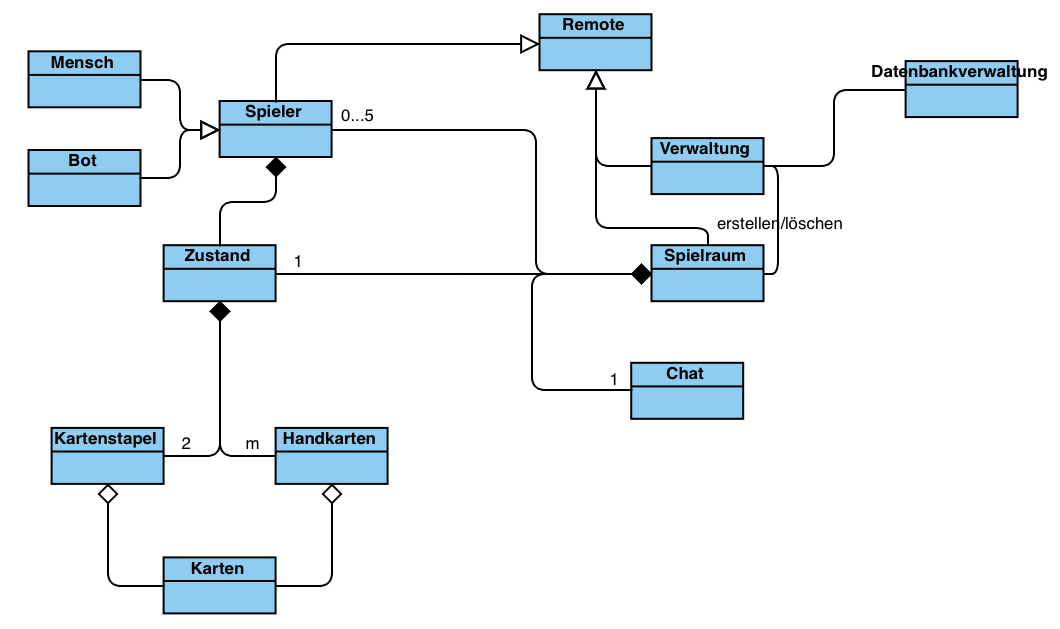
\includegraphics[scale=0.4]{../img/Analysemodel.jpg}
			\label{fig:anal}
        \end{figure}

    \clearpage

    \section{Klassendiagramme}
        Um die Implemtierung zu erleichtern haben wir das Analysemodel verfeinert und
        alle Klassen mit ihren Methoden in Klassendiagrammen dargestellt.
        Später soll es für fast jede Klasse im Diagramm ein Interface geben.
        Bei der Implemtierung ist darauf zu achten, dass manche Methoden (von Klassen die Remote implementieren) syncronized sein müssen.
        Dies ist nicht dargestellt, da Interfacemethoden diese Eigenschaft nicht haben können.
        Eine Überischt kann mittels des Paketdiagramms \ref{fig:paket} gewonnen werden.

        \begin{figure}[h]
			\centering
			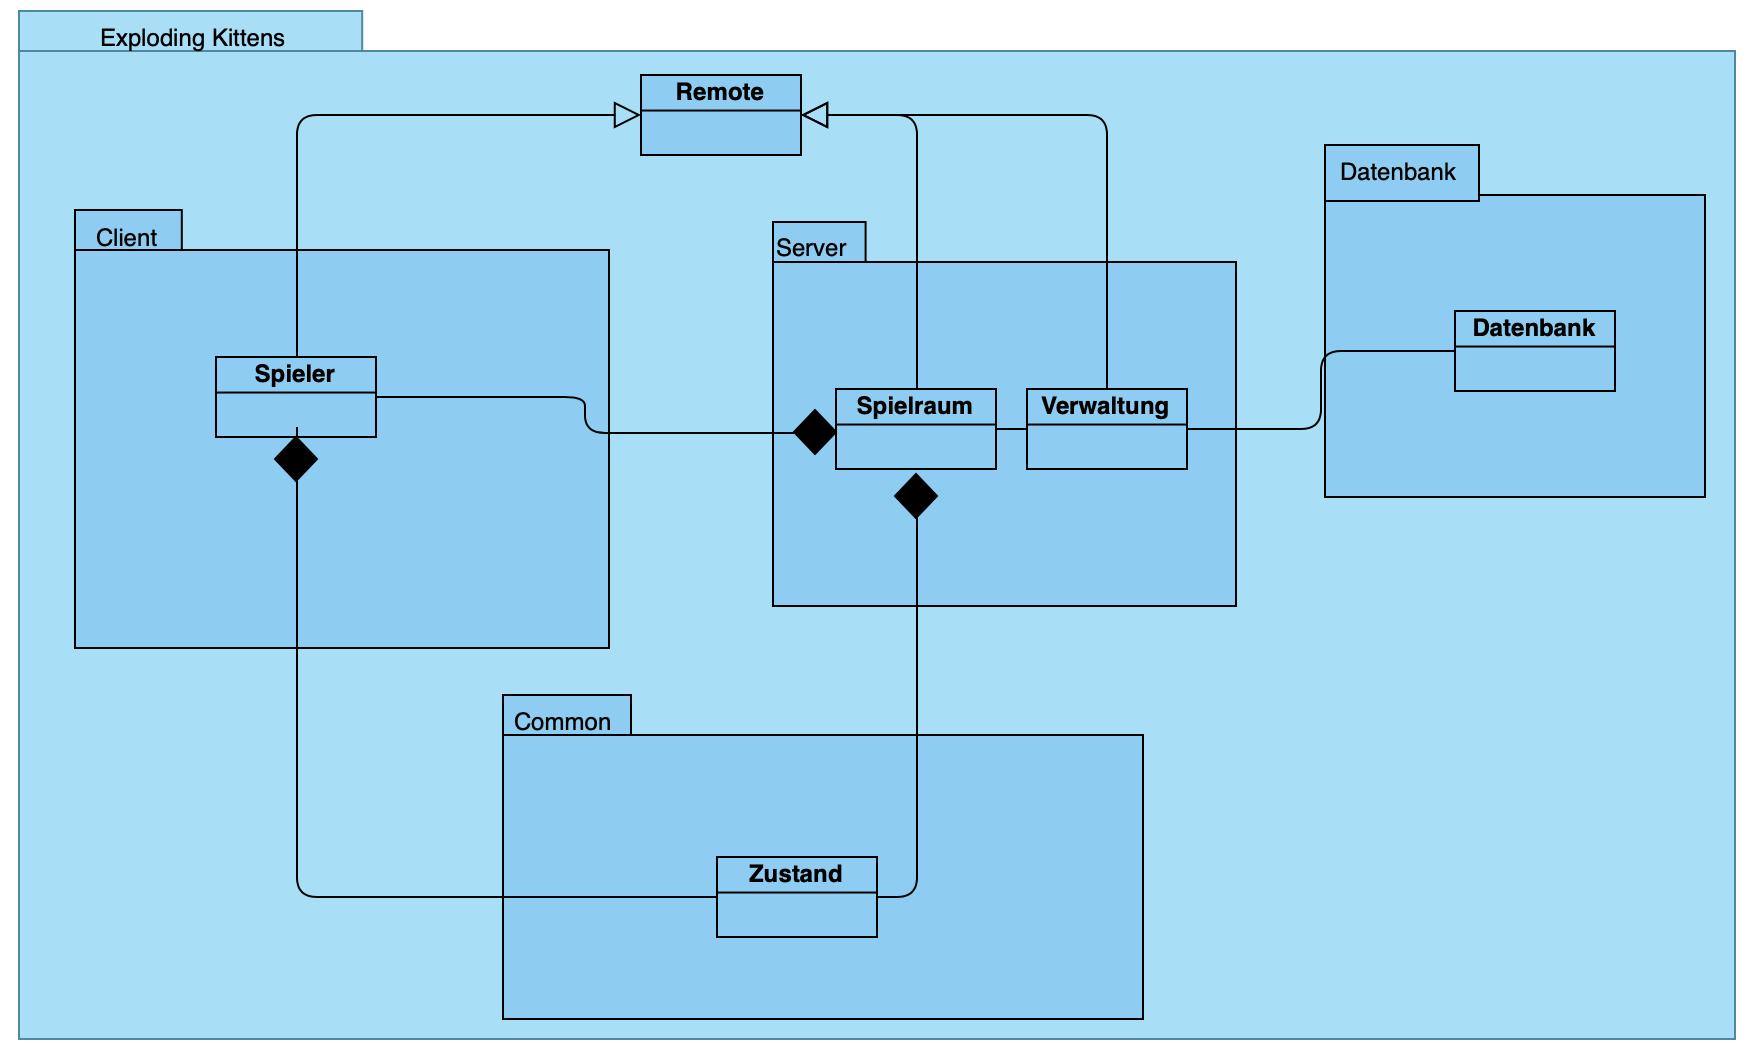
\includegraphics[scale=0.5]{../img/Klassen_Diagram/Paketdiagramm.png}
			\caption{Neben Klassen in Client- und Serverpaketen gibt es auch Klassen, die von beiden Seiten gebraucht werden. Diese Klassen befinden sich im Paket Common.}
			\label{fig:paket}
        \end{figure}

        \begin{figure}[h]
			\centering
			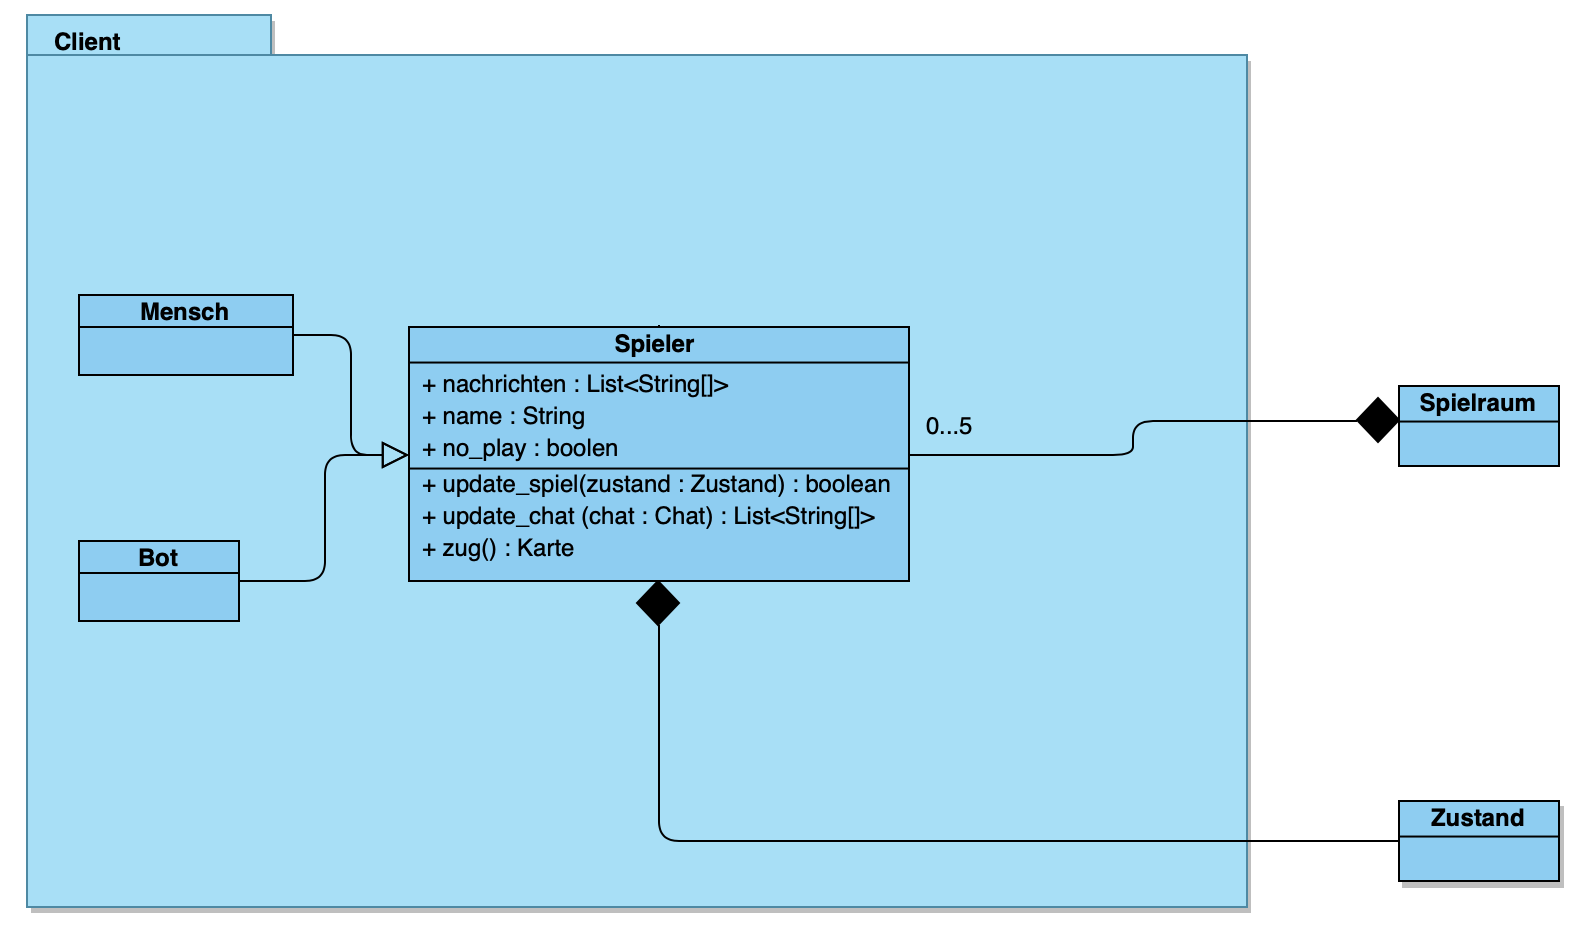
\includegraphics[scale=0.5]{../img/Klassen_Diagram/Client.png}
			\caption{Clientseitig ist vor allem die abstakte Klasse Spieler wichtig, die von Bots und Menschen implementiert wird}
        \end{figure}
        
        \begin{figure}[h]
			\centering
			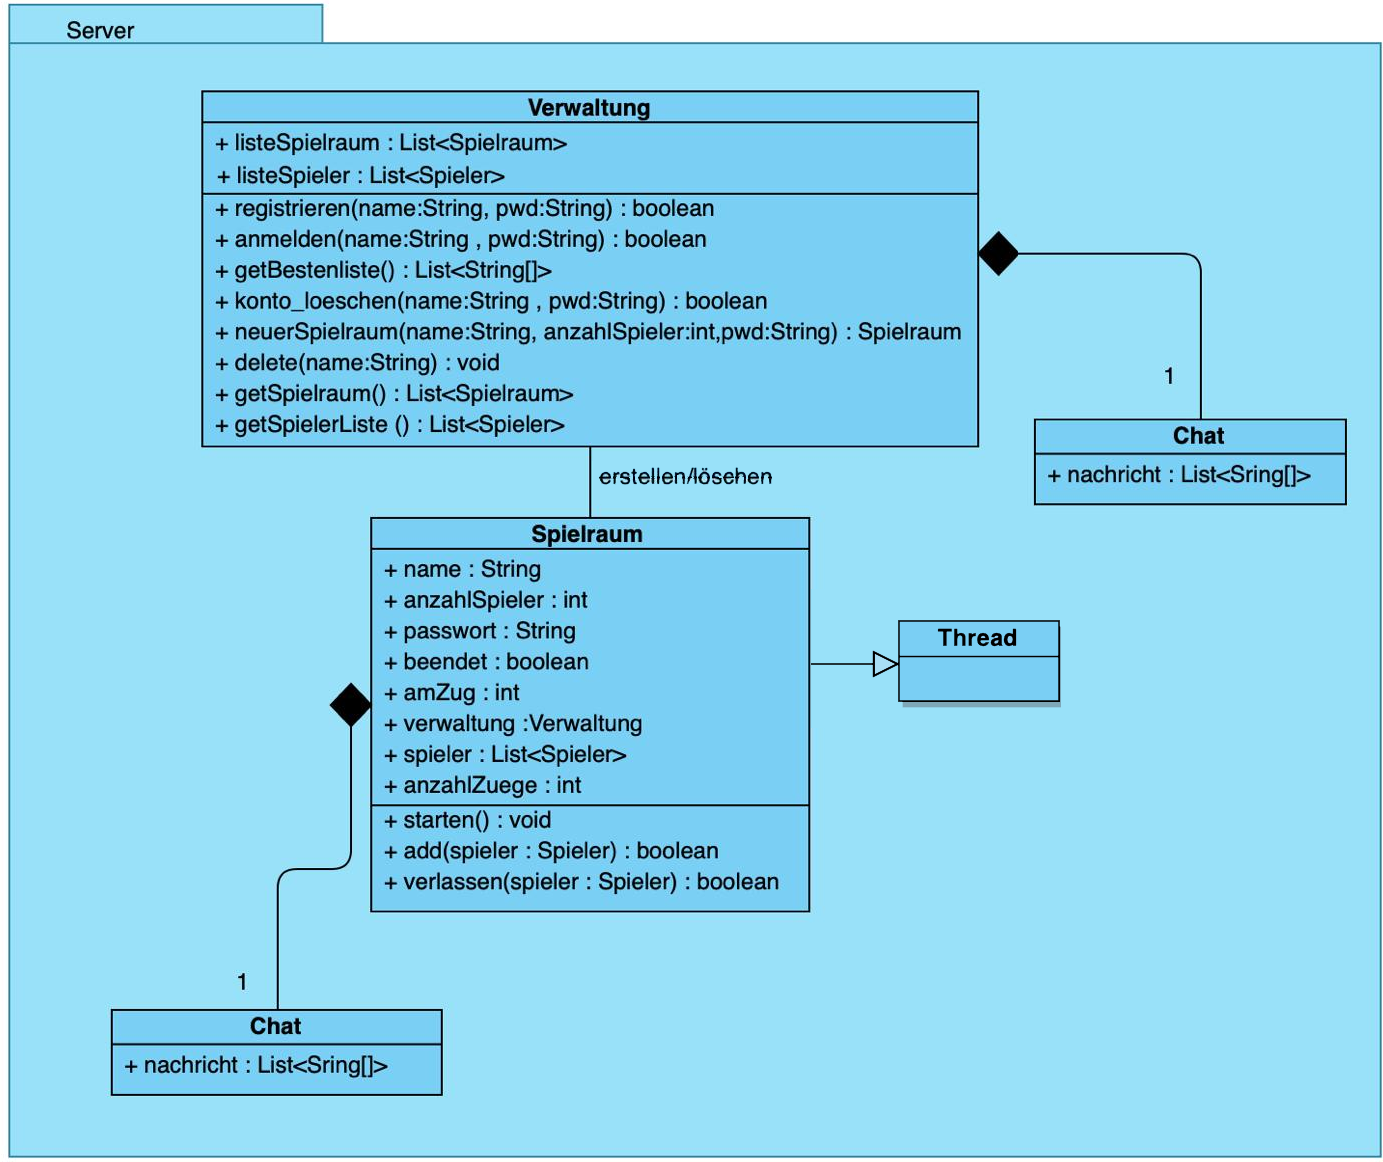
\includegraphics[scale=0.45]{../img/Klassen_Diagram/Server.png}
            \caption{Neben einer Verwaltung, die allgemeine Aufgabe wie Login übernimmt, ist der Spielraum als Leiter des Spiels wichtig. Mehrere Spielräume können parallel laufen.}
        \end{figure}

        \begin{figure}[h]
			\centering
			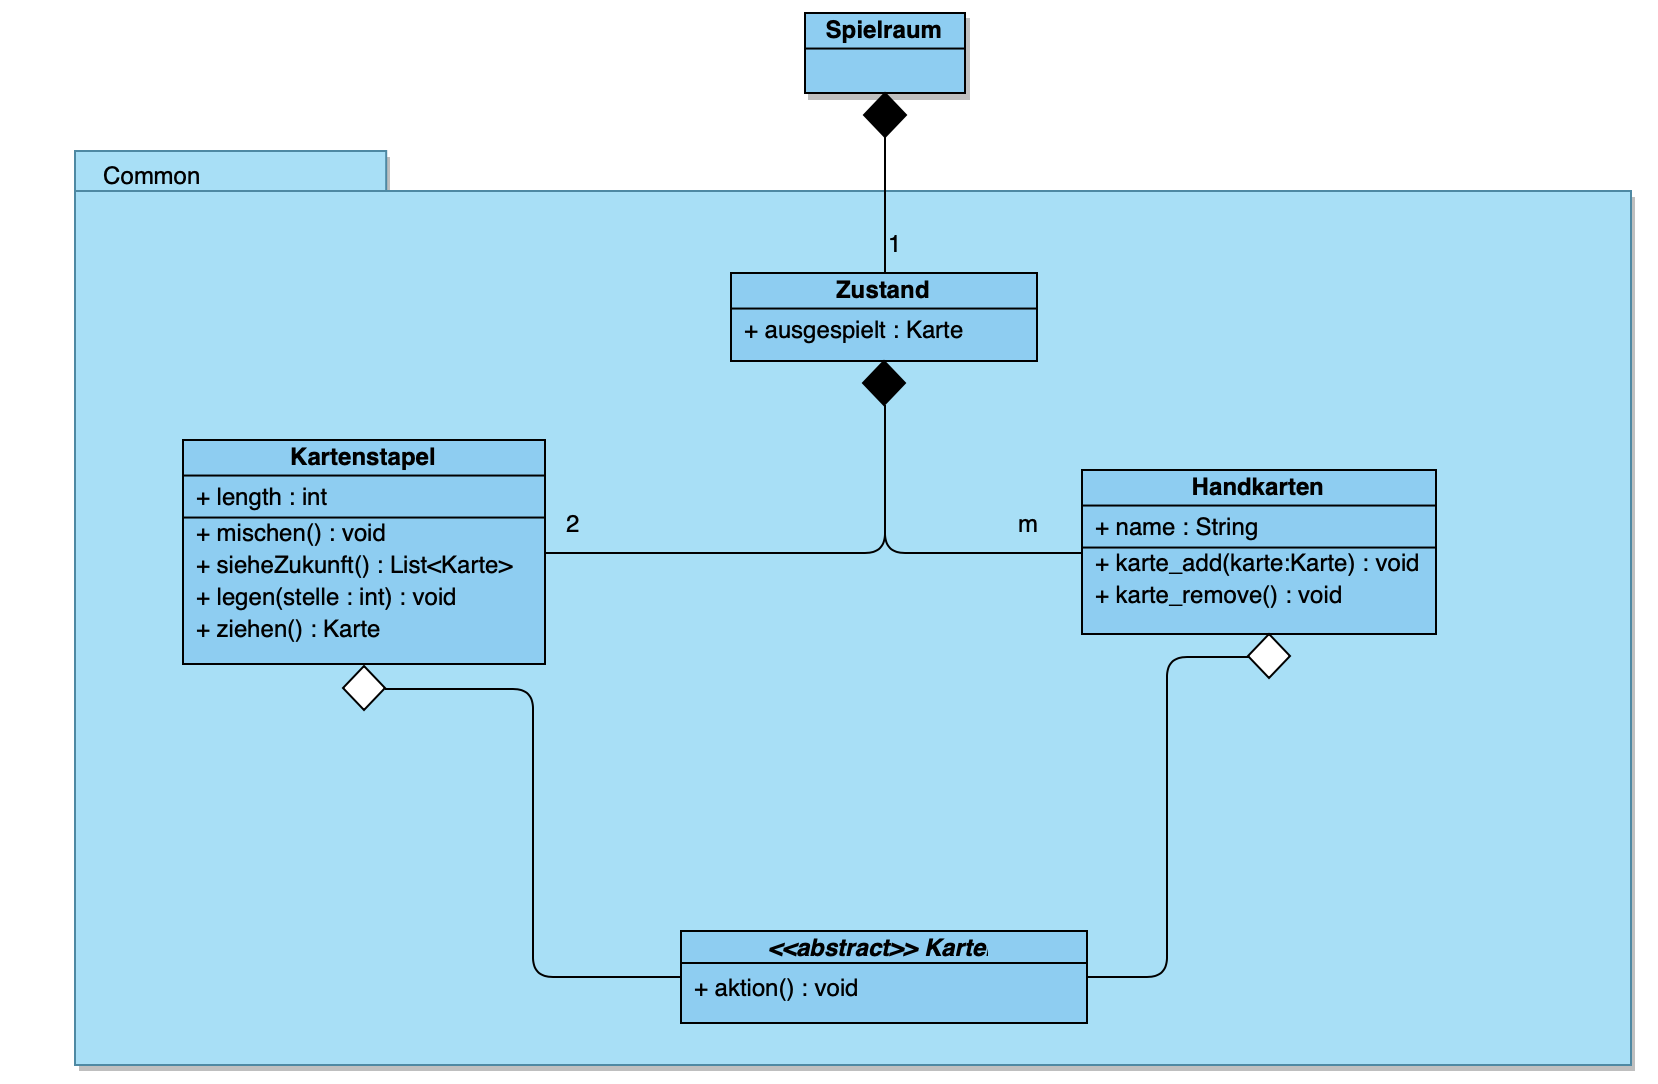
\includegraphics[scale=0.45]{../img/Klassen_Diagram/Common.png}
            \caption{Die Spiellogik wird von beiden Seiten benötigt. Es gibt keine direkten Instanzen von Karte, siehe \ref{fig:katze}}
        \end{figure}

        \begin{figure}[h]
			\centering
			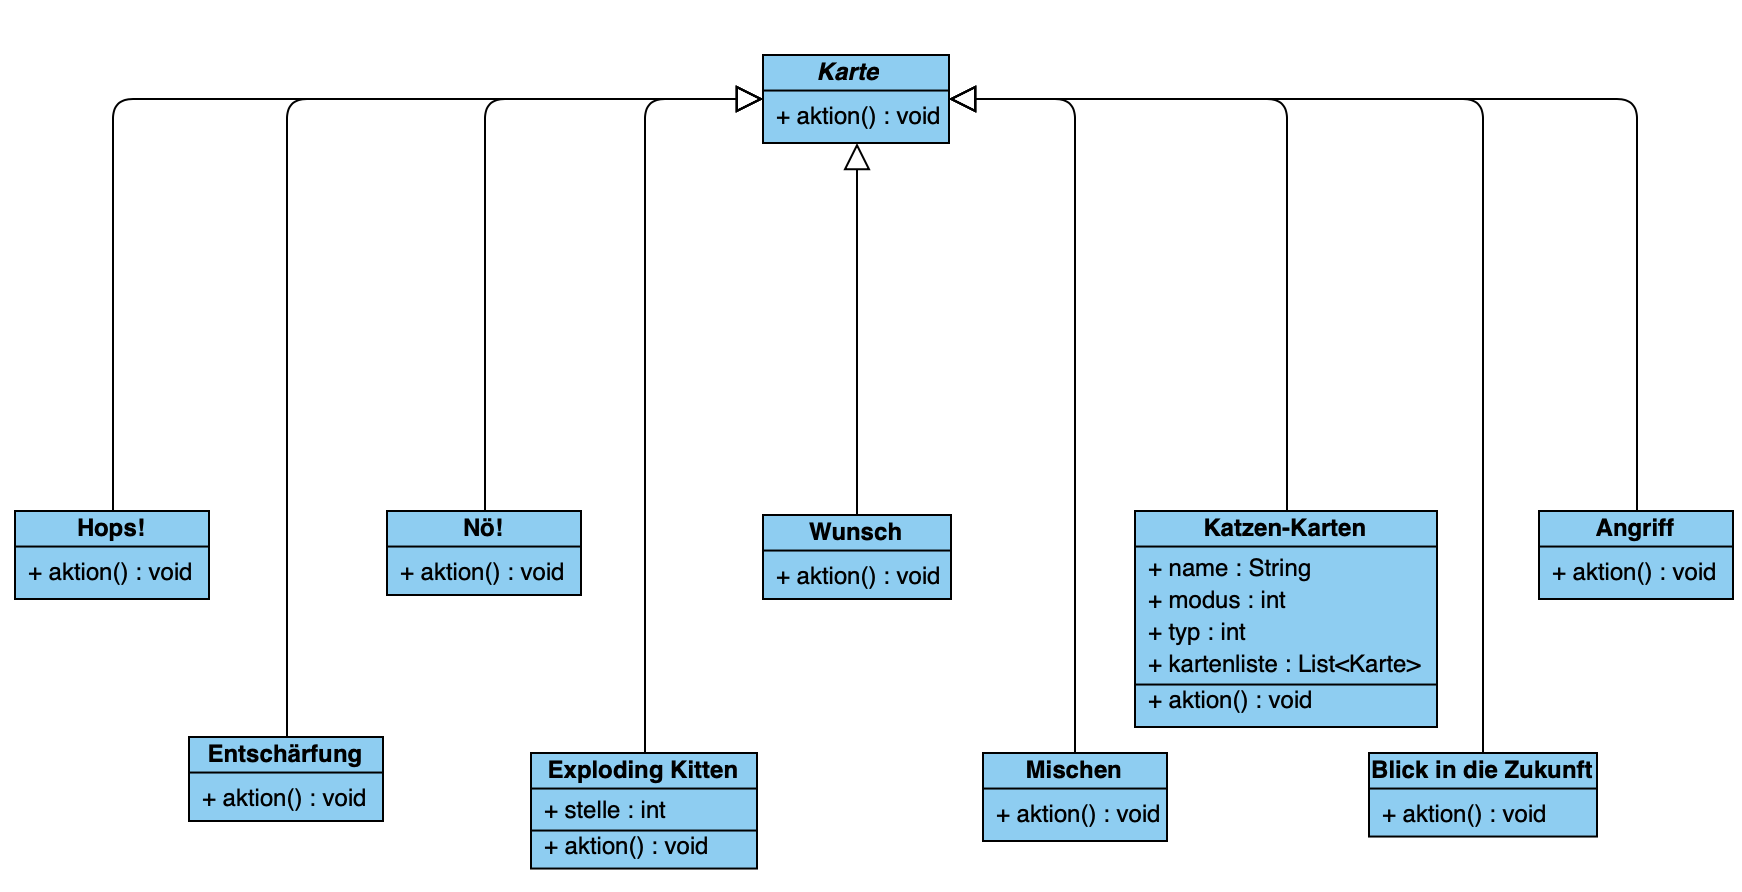
\includegraphics[scale=0.45]{../img/Klassen_Diagram/Karten.png}
            \caption{Alle Kartenarten erben von Karte. Da die Methode \textit{zug()} von \textit{Spieler} eine \textit{Karte} zurückgibt, wir aber auch Kombinationen und das Zurücklegen einer Exploding Kitten modellieren,
                haben die jeweiligen Karten Attribute die für das Ausführen der jeweiligen Aktion relevant sind.}
            \label{fig:katze}
        \end{figure}

        \begin{figure}[h]
			\centering
			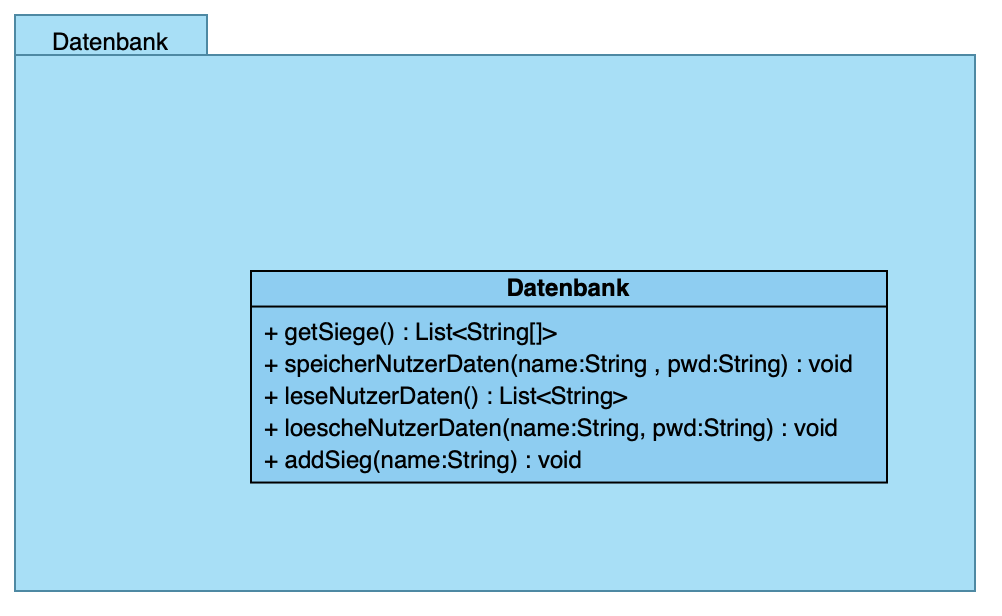
\includegraphics[scale=0.7]{../img/Klassen_Diagram/Datenbank.png}
            \caption{Die Verwaltung von Nutzerdaten und Bestenlsiten wird von einem Paket geregelt, das mit JDBC zwei SQL Tabellen verwaltet.}
        \end{figure} 
        
    \clearpage

    \section{Sequenzdiagramme} \label{sec:seq}
        Um einen besseren Überblick über den Ablauf des Spiels, die Funktionsweise von \textit{Spielraum} und die Kommunikation von Client und Server sind
        der Ablauf eiener Runde, sowie beispielshaft einige Interaktion mit der \textit{Verwaltung} als Sequenzdiagramm dargestellt.
        Für genauere Angabe über die Fehler siehe \ref{exc}

        \begin{figure}[h]
			\centering
			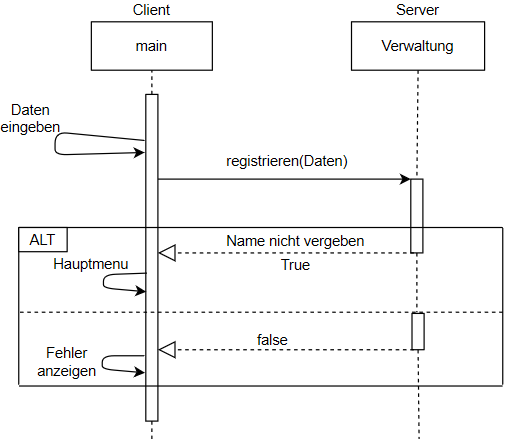
\includegraphics[scale=0.8]{../img/Sequenz_Diagramm/reg.png}
            \caption{Falls bei der Interaktion keine Antwort kommt wird ein \textit{NameFalsch} Fehler geworfen}
        \end{figure}

        \begin{figure}[h]
			\centering
			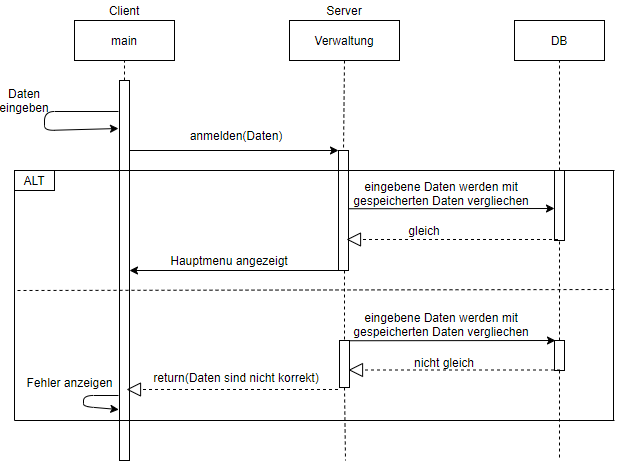
\includegraphics[scale=0.8]{../img/Sequenz_Diagramm/anmelden.png}
            \caption{Anmeldeprozess, man kommt nur mit den richtigen Daten ins Hauptmenu, sonst gibt es einen \textit{PasswortFalsch} Fehler}
        \end{figure}

        \begin{figure}[h]
			\centering
			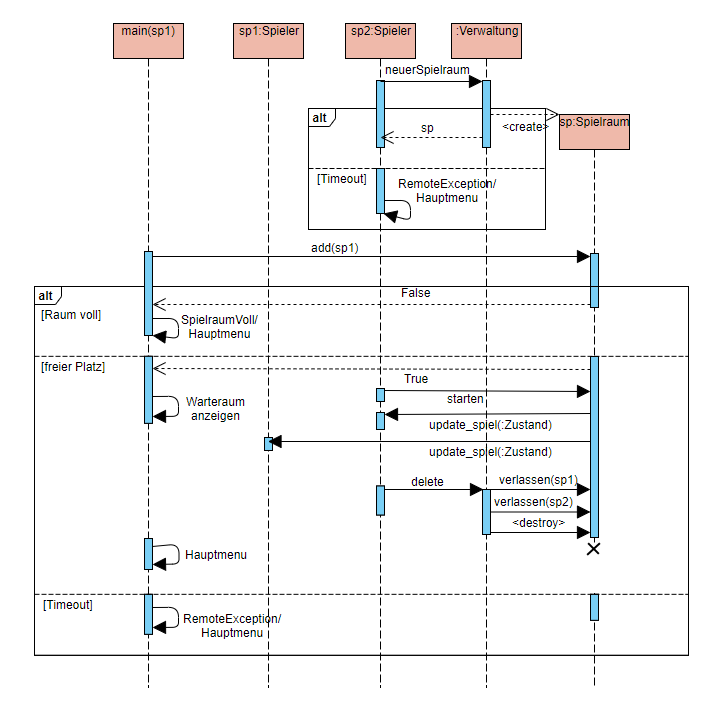
\includegraphics[scale=0.75]{../img/Sequenz_Diagramm/spielraum.png}
            \caption{Erstellen, beitretten und Löschen eines Spielraums, sowie starten und beenden des Spiels. \\
                Grundsätzlich gibt es bei jeder Kommunikation zwischen Server und Client die Möglichkeit einer \textit{RemoteException}, der Übersicht halber aber nur für das Erstellen und Beitretten eingezeichnet (auch bei folgenden Diagrammen wurde das weggelassen). \\
                Streng genommen kommen die Aufrufe von z.B. \textit{starten} aus der \textit{main/GUI}, das darzustellen wäre aber unnötig unübersichtlich.}
        \end{figure}

        \begin{figure}[h]
			\centering
            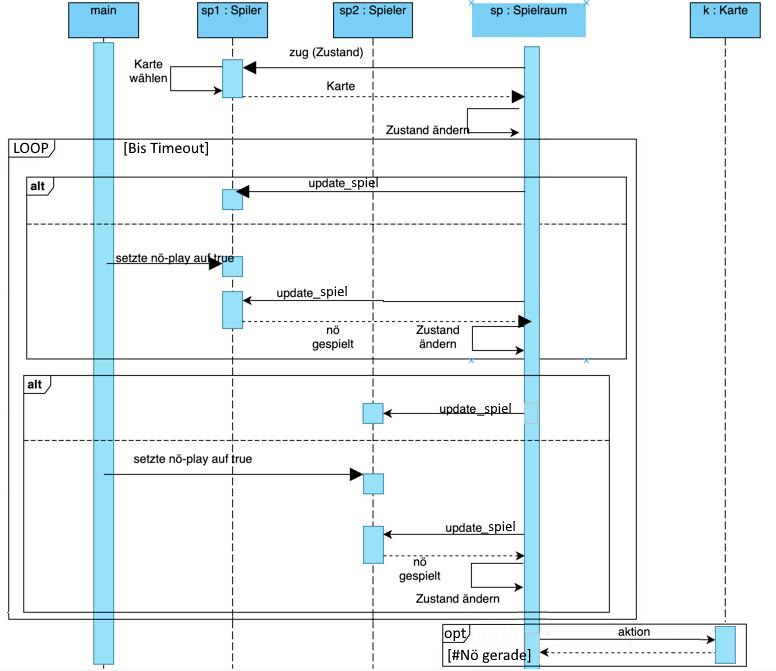
\includegraphics[scale=0.7]{../img/Sequenz_Diagramm/karte.png}
            \caption{Grundbaustein des Spiels - Das Legen einer Karte. \\
                    Dies geht nur als Antwort auf \textit{zug}, dann wird der Zug bei anderen Spieler per \textit{update\_spiel} angezeigt. Nun wird gewartet, ob ein anderer Spieler optional ein Nö spielen will. Die jeweilige GUI setzt dazu ein Attribut in \textit{sp1/sp2}.}
        \end{figure}

        \begin{figure}[h]
			\centering
			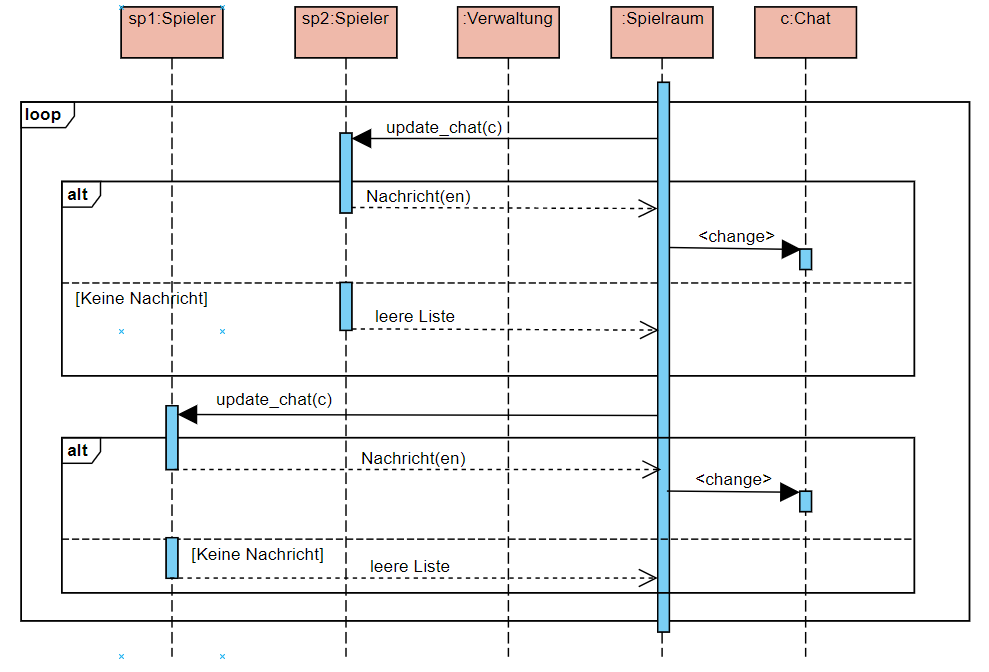
\includegraphics[scale=0.5]{../img/Sequenz_Diagramm/chat.png}
            \caption{Chatfunktionen \\
                Spieler wird nicht aktiv sondern gibt nach dem Aufruf von \textit{update\_chat} alle im Puffer liegenden Nachrichten zurück.}
        \end{figure}

    \clearpage

    \section{Exceptions} \label{exc}
        Die in \ref{sec:seq} erwähnten Fehler/\textit{Exceptions} sind hier nochmal in einem Klassendiagramm verdeutlicht:
        \begin{figure}[h]
			\centering
			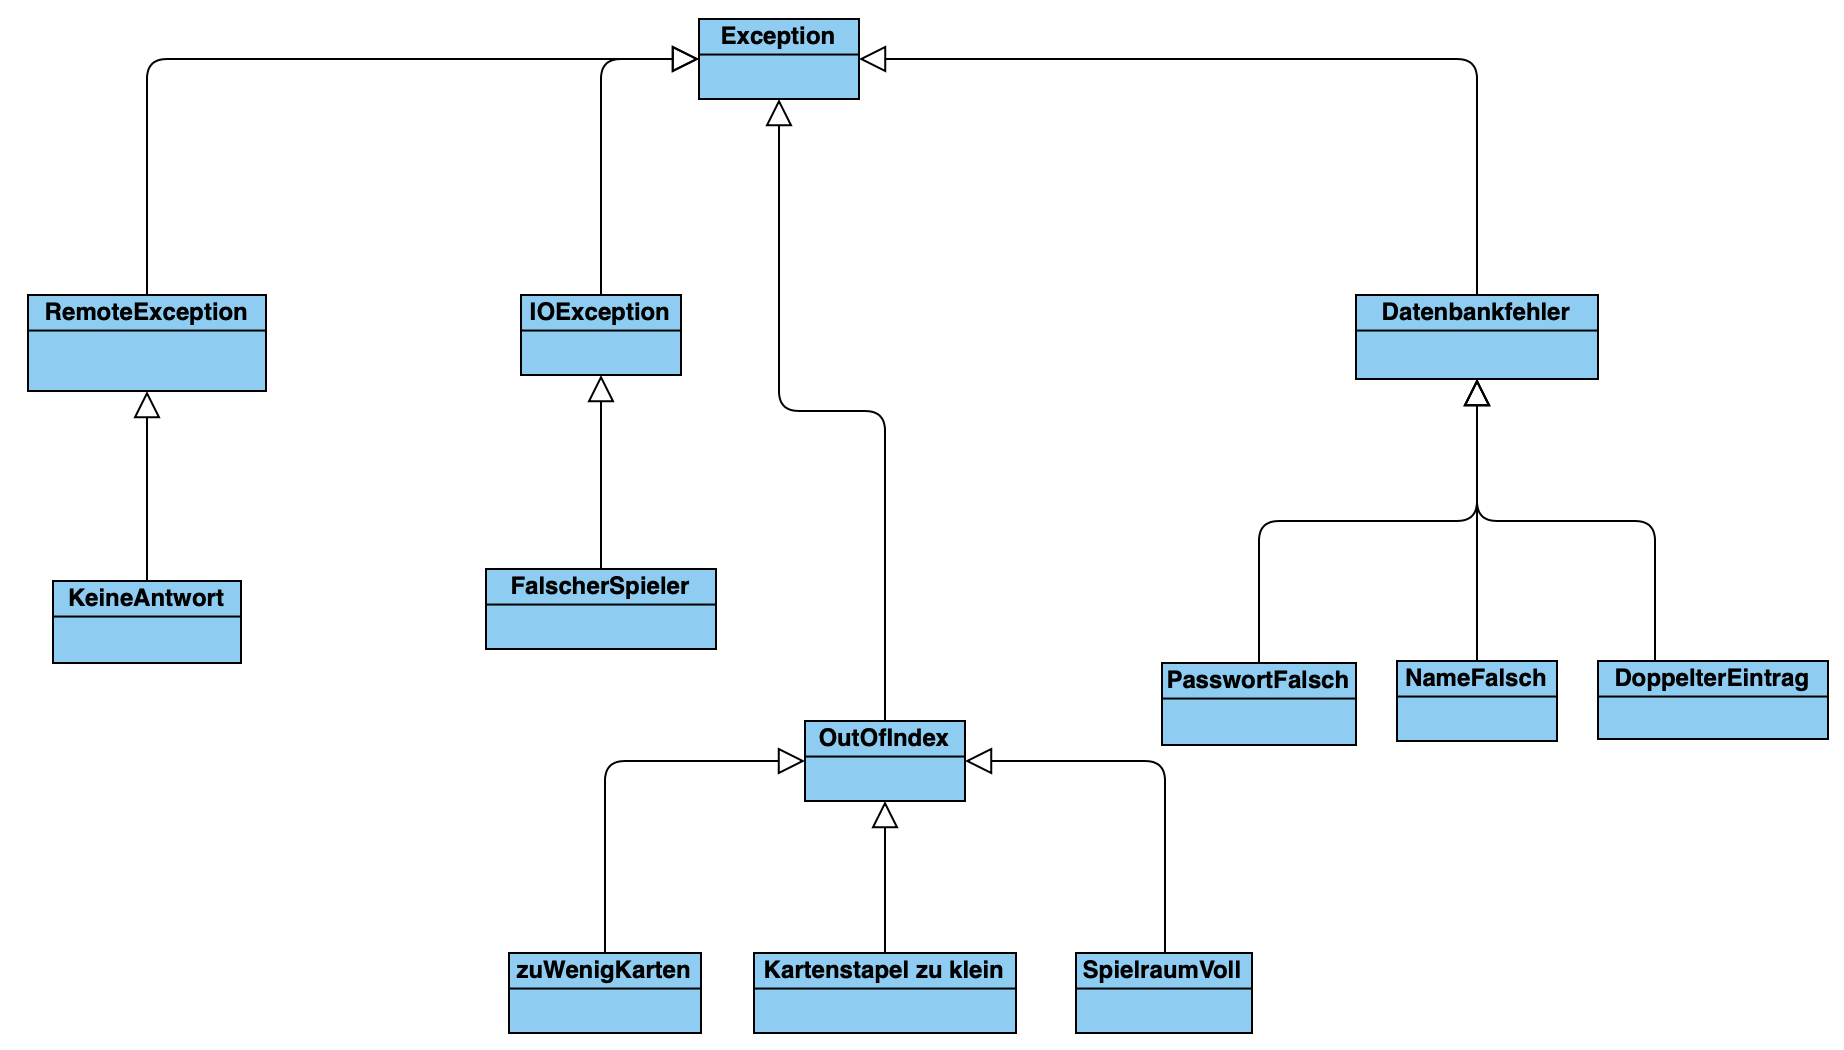
\includegraphics[scale=0.4]{../img/Exceptions.png}
            \caption{Wir unterteilen unter anderem zwischen Verbindungsfehlern (\textit{RemoteException}), Fehlern in der Spiellogik (\textit{OutOffIndex}) und \textit{Datenbankfehlern}}
        \end{figure} 
    \clearpage

    \section{Bot}

        \begin{figure}[h]
            \centering
            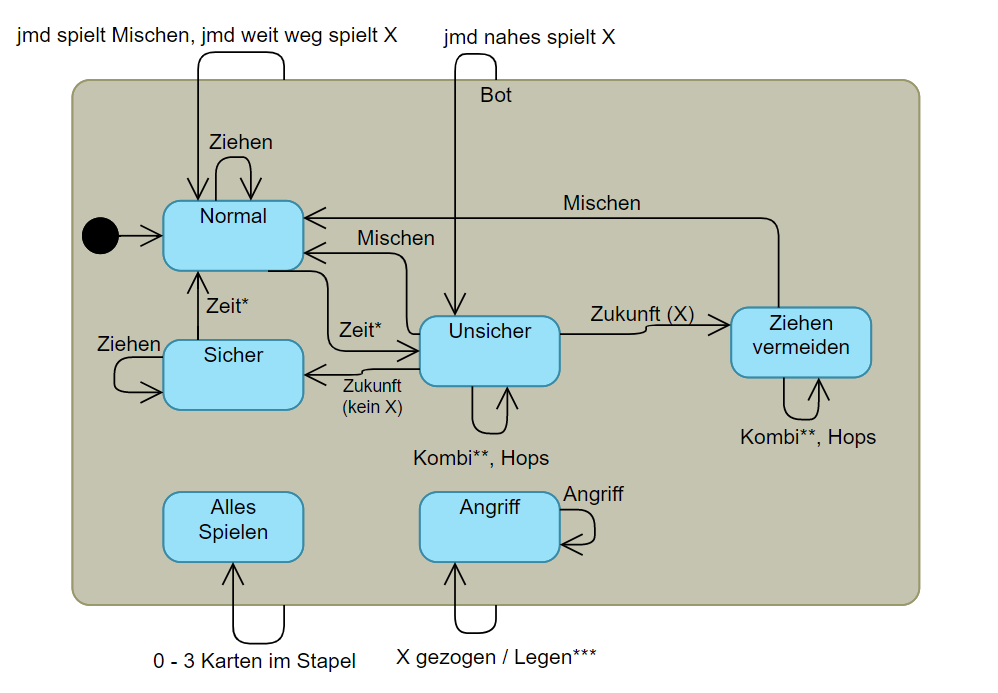
\includegraphics[scale=0.5]{../img/bot.png}
            \caption{Zustandsgraph des Computers}
            \label{fig:bot}
        \end{figure}

        Das Konzept unseres Computergegners basiert auf einem Zustandsgraphen, der in \ref{fig:bot} gezeigt ist.
        Generell gilt, dass sobald eine Aktion eines anderen Spieler durchgeführt wird, der Zustand unseres Bots angepasst werden kann
        (Wir erhalten diese Information über einen Aufruf von \textit{update\_spiel}). Falls wir mit der Methode \textit{zug} zu einem Zug aufgefordert werden,
        wählen wir die Möglichkeiten in unserem aktuellen Zug, die die höchste Priorität hat. \\
        Beispielsweise haben wir im Zustand \textit{Sicher} eine \textit{Blick-in-die-Zukunft} und eine \textit{Mischen} Karte (beide wären zulässig), so
        spielen wir \textit{Blick-in-die-Zukunft}, da diese Karte die höchste Priorität hat. Die Prioritäten sind global festgelegt, von höchste zur niedrigen Priorität haben wir:\\

        \textit{Blick-in-die-Zukunft, Mischen, Hops, Kombination, Ziehen}\\
    
        Falls in einem Zustand keine der möglichen Karten vorhanden sind muss der Bot ziehen.\\
        Wir unterscheiden eine einfache Variante und eine komplexere Variante. Die Unterscheide liegen in der Umsetzung der Übergänge und Aktionen
        \textit{Zeit, Kombi} und \textit{Legen}:\\

        \begin{enumerate}
            \item [Zeit] \textit{einfach:} alle 2 Runden\\
                \textit{komplex:} In Abhängigkeit von $\frac{\#X}{\#Karten im Stapel}$, also der Chance auf eine Exploding Kitten.
            \item [Legen] \textit{einfach:} Immer an die erste Stelle\\
                \textit{komplex:} Mit bestimmten Wahrscheinlichkeiten an Stelle 1,2,3 oder zufällig.
            \item [Kombi] \textit{einfach:} nur 2er Kombinationen\\
                \textit{komplex:} Sparen auf 3er/5er Kombinationen, in Abhängigkeit von eigenen $\#Handkarten$ und der Chance auf eine Exploding Kitten. Die Wahl des Opfers hängt ebenfalls von den jeweiligen $\#Handkarten$ ab.
        
        \end{enumerate}

        Die komplexe Variante entscheidet in Abhängigkeit von \textit{\#Handkarten} und Position auf des Spielers bei welchem Spieler ein \textit{Nö} gespielt wird.

    \clearpage

    \section{Gantt Diagramm}
        Für die Plannung des weiteren Vorgehens wurden alle Aufgaben der Implementierung und Optimierung benannt und in einem Gantt Diagram visualisiert.

        \begin{figure}[h]
			\centering
			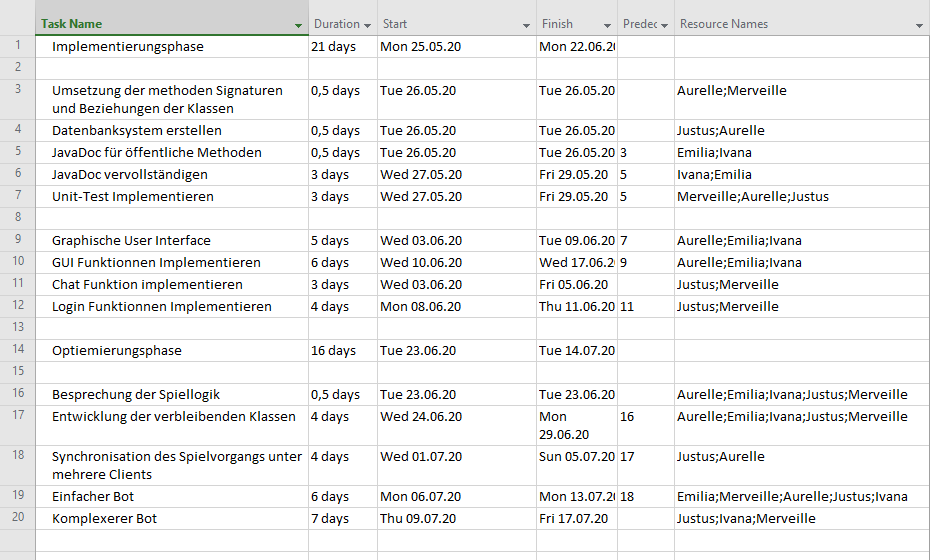
\includegraphics[scale=0.6]{../img/Gantt_Diagramm/task.png}
            \caption{Alle zu erledigende Aufgaben}
            \label{fig:auf}
        \end{figure} 

        \begin{figure}[h]
			\centering
			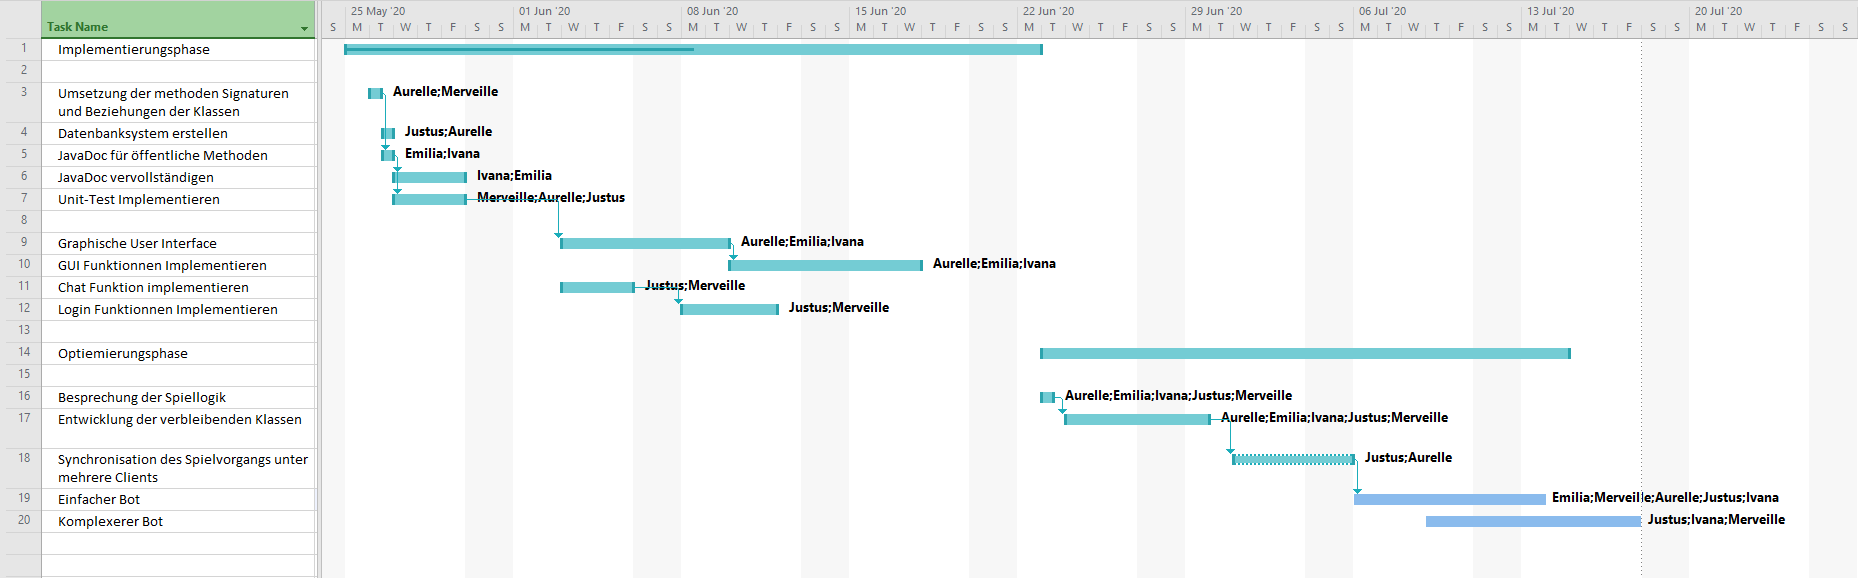
\includegraphics[scale=0.3]{../img/Gantt_Diagramm/task_and_graph.png}
            \caption{Visualisierung der Aufgaben in \ref{fig:auf}. Besser lesbar in \ref{fig:gantt}}
        \end{figure} 

        \begin{figure}[h]
			\centering
			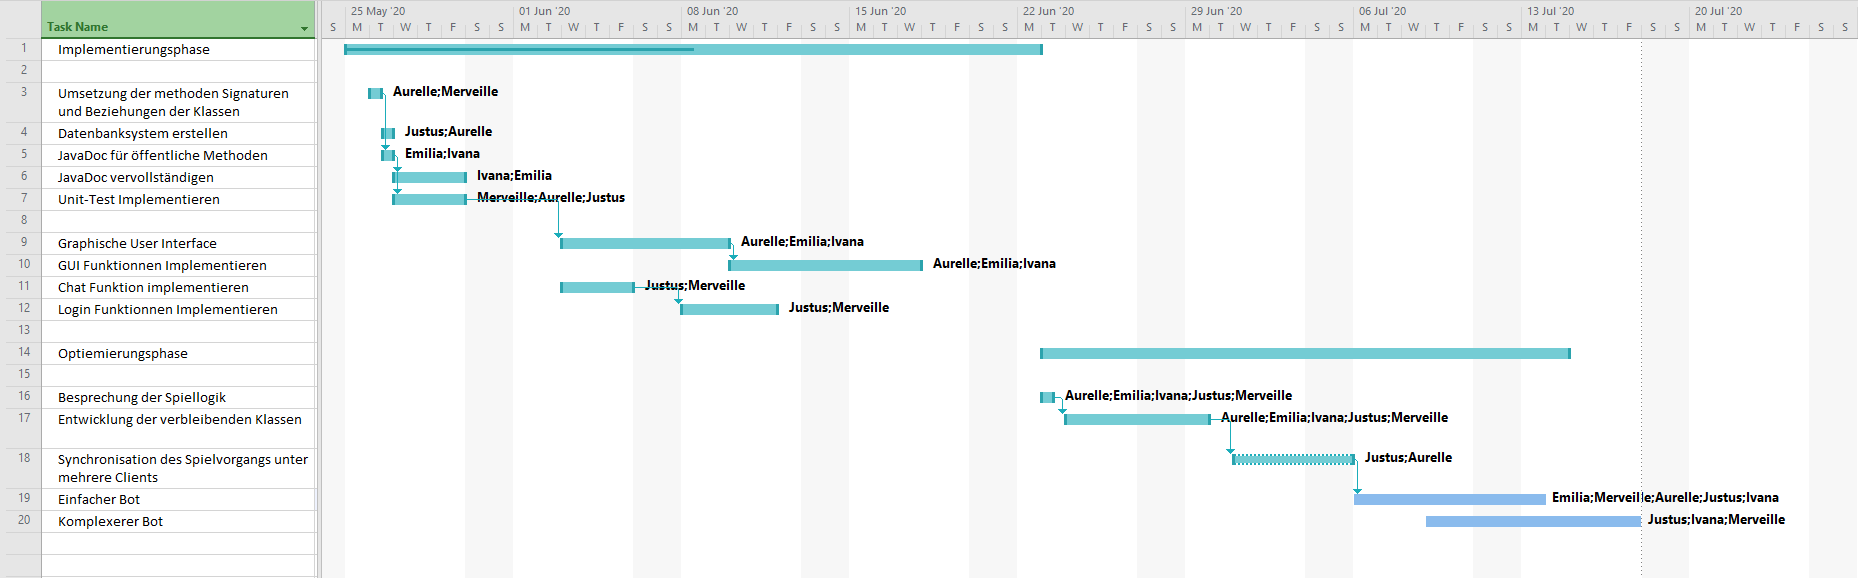
\includegraphics[scale=0.5, angle=-90]{../img/Gantt_Diagramm/task_and_graph.png}
        \end{figure}
        \label{fig:gantt}

\end{document}}